% Gabarit pandoc des corrigés publiés (brut et guidé). Contenu sans marque ni nom de site.
% Compilation : lualatex (latexmk -lualatex).
% Le Markdown reste la source unique : ne pas éditer ce fichier .tex à la main.
\documentclass[11pt,a4paper]{article}

% --- Moteur, polices (Latin Modern) et langue ---------------------------------
\usepackage{iftex}
\ifLuaTeX\else\errmessage{Ce document se compile avec lualatex}\fi
\usepackage{amsmath,amssymb,mathtools}
\usepackage{fontspec}
% mathrm=sym : \mathrm prend ses glyphes dans la police mathématique (ℓ, μ, Ω), comme KaTeX.
\usepackage[math-style=TeX,bold-style=TeX,mathrm=sym]{unicode-math}
% Repli pour les glyphes absents de Latin Modern (indices et exposants Unicode,
% flèches, filets des schémas en texte, symboles) : DejaVu, puis Latin Modern Math
% (ℓ, lettres mathématiques Unicode des légendes).
\directlua{
  luaotfload.add_fallback("repliTexte", {"DejaVuSerif:mode=harf;", "DejaVuSans:mode=harf;", "file:latinmodern-math.otf:mode=harf;"})
  luaotfload.add_fallback("repliMono", {"DejaVuSansMono:mode=harf;", "DejaVuSans:mode=harf;", "file:latinmodern-math.otf:mode=harf;"})
}
\setmainfont{Latin Modern Roman}[RawFeature={fallback=repliTexte}]
\setsansfont{Latin Modern Sans}[RawFeature={fallback=repliTexte}]
\setmonofont{Latin Modern Mono}[RawFeature={fallback=repliMono}]
\setmathfont{Latin Modern Math}
\usepackage[french]{babel}
\frenchsetup{SmallCapsFigTabCaptions=false}

% --- Mise en page --------------------------------------------------------------
\usepackage[a4paper,margin=2.2cm,headheight=14pt,footskip=1.2cm]{geometry}
\usepackage{microtype}
\setlength{\emergencystretch}{4em}
\tolerance=1500
\setlength{\parindent}{0pt}
\setlength{\parskip}{0.55\baselineskip plus 2pt minus 1pt}
\usepackage{xcolor}
% Gris nommés : babel-french rend « ! » actif dans le document.
\definecolor{gris2}{gray}{0.98}
\definecolor{gris3}{gray}{0.97}
\definecolor{gris5}{gray}{0.95}
\definecolor{gris35}{gray}{0.65}
\definecolor{gris40}{gray}{0.60}
\definecolor{gris45}{gray}{0.55}
\definecolor{gris50}{gray}{0.50}
\definecolor{gris55}{gray}{0.45}
\definecolor{gris60}{gray}{0.40}
\definecolor{gris65}{gray}{0.35}
\definecolor{gris70}{gray}{0.30}
\definecolor{gris80}{gray}{0.20}
\definecolor{gris85}{gray}{0.15}
\usepackage{graphicx}
\usepackage{float}
\usepackage{caption}
\captionsetup{font=small,labelformat=empty,justification=centering}
\usepackage{booktabs,longtable,array,multirow,calc}
\usepackage{siunitx}
\sisetup{locale=FR}
\usepackage[version=4]{mhchem}
\usepackage{listings}
\usepackage{fancyhdr}
\usepackage{lastpage}
\usepackage[most]{tcolorbox}
\usepackage{enumitem}
\setlist{nosep,leftmargin=*,topsep=2pt}
\usepackage[hidelinks,unicode]{hyperref}
\usepackage{bookmark}
\hypersetup{pdftitle={Mines-Ponts MPI — Informatique 1 2026},pdfauthor={Rédigé par IA},pdfcreator={LaTeX},pdfsubject={Corrigé brut}}
\usepackage{xurl}

% --- Pandoc : listes, tableaux, figures ----------------------------------------
\providecommand{\passthrough}[1]{#1}
\providecommand{\tightlist}{\setlength{\itemsep}{0pt}\setlength{\parskip}{0pt}}

\makeatletter
\def\maxwidth{\ifdim\Gin@nat@width>\linewidth\linewidth\else\Gin@nat@width\fi}
\def\maxheight{\ifdim\Gin@nat@height>0.55\textheight 0.55\textheight\else\Gin@nat@height\fi}
\makeatother
\setkeys{Gin}{width=\maxwidth,height=\maxheight,keepaspectratio}
\setcounter{secnumdepth}{-\maxdimen}
\providecommand{\pandocbounded}[1]{#1}
\usepackage{longtable,booktabs,array}

% --- Code (listings) -----------------------------------------------------------
\lstset{
  basicstyle=\ttfamily\small,
  columns=fullflexible,
  keepspaces=true,
  breaklines=true,
  breakatwhitespace=false,
  postbreak=\mbox{\textcolor{gris50}{$\hookrightarrow$}\space},
  frame=single,
  rulecolor=\color{gris35},
  framesep=4pt,
  xleftmargin=5pt,xrightmargin=5pt,
  backgroundcolor=\color{gris3},
  keywordstyle=\bfseries,
  commentstyle=\color{gris65},
  stringstyle=\color{gris80},
  showstringspaces=false,
  tabsize=4,
  extendedchars=true,
  aboveskip=6pt,belowskip=6pt,
}

% --- Macros des corrigés (KaTeX ↔ LaTeX) ---------------------------------------
% Les corrigés sont écrits pour KaTeX : on définit ici ce que KaTeX connaît et
% que LaTeX n'a pas, sans jamais retoucher le Markdown.
\providecommand{\R}{\mathbb{R}}
\providecommand{\N}{\mathbb{N}}
\providecommand{\Z}{\mathbb{Z}}
\providecommand{\Q}{\mathbb{Q}}
\providecommand{\C}{\mathbb{C}}
\providecommand{\dd}{\mathrm{d}}
\providecommand{\llbracket}{\lBrack}
\providecommand{\rrbracket}{\rBrack}
\providecommand{\lBrace}{\lbrace}
\providecommand{\rBrace}{\rbrace}
\providecommand{\Box}{\square}
\providecommand{\Diamond}{\lozenge}
\providecommand{\varnothing}{\emptyset}
\providecommand{\argmax}{\operatorname*{arg\,max}}
\providecommand{\argmin}{\operatorname*{arg\,min}}
\renewcommand{\leq}{\leqslant}
\renewcommand{\geq}{\geqslant}

% Équation hors texte : réduite à la largeur de la ligne si elle déborde.
\newsavebox{\boiteequation}
\newcommand{\equationajustee}[1]{%
  \sbox{\boiteequation}{$\displaystyle #1$}%
  \ifdim\wd\boiteequation>\linewidth
    \[\resizebox{\linewidth}{!}{\usebox{\boiteequation}}\]%
  \else
    \[#1\]%
  \fi}

% --- Encadrés pédagogiques (sobres, lisibles en noir et blanc) -----------------
\tcbset{
  encadre/.style={
    enhanced,breakable,sharp corners,
    colback=white,colframe=gris55,
    boxrule=0.4pt,leftrule=2.2pt,
    left=6pt,right=6pt,top=3pt,bottom=3pt,
    before skip=6pt,after skip=6pt,
    fonttitle=\bfseries\small,coltitle=black,
    attach title to upper,after title={\quad},
    parbox=false,
  }
}
\newtcolorbox{indication}[1]{encadre,colframe=gris45,colback=gris2,title={Indication~#1}}
\newtcolorbox{methode}{encadre,colframe=gris70,title={Méthode}}
\newtcolorbox{piege}{encadre,colframe=gris85,boxrule=0.8pt,leftrule=2.2pt,title={Piège}}
\newtcolorbox{jury}{encadre,colframe=gris60,colback=gris5,title={Jury}}
\newtcolorbox{encadrenote}{encadre,colframe=gris40}

% --- Titres de section ---------------------------------------------------------
\usepackage{titlesec}
\titleformat{\section}{\Large\bfseries}{}{0pt}{}
\titleformat{\subsection}{\large\bfseries}{}{0pt}{}
\titleformat{\subsubsection}{\normalsize\bfseries}{}{0pt}{}
\titlespacing*{\section}{0pt}{14pt plus 4pt minus 2pt}{6pt}
\titlespacing*{\subsection}{0pt}{10pt plus 3pt minus 2pt}{4pt}
\titlespacing*{\subsubsection}{0pt}{8pt plus 2pt minus 2pt}{2pt}

% --- En-tête et pied de page ---------------------------------------------------
\pagestyle{fancy}
\fancyhf{}
\fancyhead[L]{\small\textsc{Corrigé brut} · Mines-Ponts MPI}
\fancyhead[R]{\small Informatique 1 2026}
\fancyfoot[L]{\footnotesize Corrigé rédigé par IA, non officiel}
\fancyfoot[R]{\footnotesize \thepage\,/\,\pageref*{LastPage}}
\renewcommand{\headrulewidth}{0.4pt}
\renewcommand{\footrulewidth}{0pt}
\fancypagestyle{plain}{\fancyhf{}\fancyfoot[R]{\footnotesize \thepage\,/\,\pageref*{LastPage}}\fancyfoot[L]{\footnotesize Corrigé rédigé par IA, non officiel}\renewcommand{\headrulewidth}{0pt}}

\begin{document}
\thispagestyle{plain}
\begin{center}
  {\small\scshape Corrigé brut}\par\smallskip
  {\LARGE\bfseries Mines-Ponts MPI — Informatique 1 2026\par}\medskip
  {\large Mines-Ponts · MPI · Informatique 1 · 2026\par}
\end{center}
\vspace{2pt}\hrule\vspace{8pt}

\emph{Corrigé rédigé par IA, non officiel. Signalez toute erreur.}

Conventions.

\begin{itemize}
\tightlist
\item
  Une lettre de \(\Sigma_2\) est notée \(\binom{a}{b}\) ; une lettre de \(\Sigma_3\) est notée \(\langle a,b,c\rangle\) (composantes des lignes 1, 2, 3, de haut en bas).
\item
  La lettre nulle de \(\Sigma_n\) est notée \(\mathbf{0}\).
\item
  Les lignes sont numérotées de \(1\) à \(n\) comme dans l'énoncé ; la ligne \(i\) correspond à l'indice \texttt{i-1} du tableau OCaml.
\item
  Pour un automate \(\mathcal{A}\), \(\widehat{\delta}(q,m)\) désigne l'ensemble des états atteints depuis \(q\) en lisant le mot \(m\).
\item
  Les opérations arithmétiques coûtent \(O(1)\) (hypothèse de l'énoncé : entiers aussi grands qu'on veut).
\item
  Pour un mot \(u\) sur \(\{0,1\}\), on utilise sans le redire que \textbf{à longueur fixée, \(u\) est déterminé par \(v(u)\)} (unicité de l'écriture binaire, voir Q2).
\end{itemize}

\hypertarget{impluxe9mentation-de-quelques-fonctions-utiles}{%
\section{1. Implémentation de quelques fonctions utiles}\label{impluxe9mentation-de-quelques-fonctions-utiles}}

\hypertarget{question-1}{%
\subsection{Question 1}\label{question-1}}

\begin{lstlisting}[language=Caml]
(* pow2 n = 2^n, exponentiation rapide *)
let rec pow2 n =
  if n = 0 then 1
  else
    let p = pow2 (n / 2) in
    if n mod 2 = 0 then p * p else 2 * p * p
\end{lstlisting}

\textbf{Correction.} Récurrence forte sur \(n\). Pour \(n=0\) on renvoie \(1=2^0\). Pour \(n\ge1\), on a \(\lfloor n/2\rfloor<n\), donc \(p=2^{\lfloor n/2\rfloor}\).

\begin{itemize}
\tightlist
\item
  Si \(n\) est pair, on renvoie \(p^2=2^n\).
\item
  Si \(n\) est impair, on renvoie \(2p^2=2^{2\lfloor n/2\rfloor+1}=2^n\).
\end{itemize}

\textbf{Complexité.} Un seul appel récursif, sur \(\lfloor n/2\rfloor\), et un nombre borné d'opérations :

\equationajustee{C(n)=C(\lfloor n/2\rfloor)+O(1).}

La suite \(n,\lfloor n/2\rfloor,\dots\) atteint \(0\) en \(\lfloor\log_2 n\rfloor+1\) étapes, d'où \(\boxed{C(n)=O(\log n)}\).

\hypertarget{question-2}{%
\subsection{Question 2}\label{question-2}}

Soit \(\psi:\Sigma_n\to\mathbb{N}\) définie par

\equationajustee{\psi\big((a_1,\dots,a_n)^{\mathsf T}\big)=\sum_{i=1}^n 2^{i-1}a_i}

(la colonne lue de haut en bas, poids faible en ligne 1, comme pour \(v\)).

\begin{itemize}
\tightlist
\item
  \(\psi\) est à valeurs dans \([\![0,2^n-1]\!]\) : \(0\le\psi(a)\le\sum_{i=1}^n2^{i-1}=2^n-1\).
\item
  \(\psi\) est injective. Si \(a\ne b\), soit \(i_0\) le plus grand indice où ils diffèrent, avec par exemple \(a_{i_0}=1\) et \(b_{i_0}=0\). Alors
\end{itemize}

\equationajustee{\begin{aligned}
\psi(a)-\psi(b)&=2^{i_0-1}+\sum_{i<i_0}2^{i-1}(a_i-b_i)\\
&\ge 2^{i_0-1}-(2^{i_0-1}-1)\\
&=1.
\end{aligned}}

\begin{itemize}
\tightlist
\item
  \(|\Sigma_n|=2^n=\big|[\![0,2^n-1]\!]\big|\) : une injection entre ensembles finis de même cardinal est une bijection.
\end{itemize}

\textbf{La bijection demandée est \(\varphi=\psi^{-1}:[\![0,2^n-1]\!]\to\Sigma_n\).}

Explicitement, \(\varphi(x)\) est la colonne dont la ligne \(i\) vaut \(\lfloor x/2^{i-1}\rfloor \bmod 2\) : le bit de poids \(2^{i-1}\) de \(x\) est placé en ligne \(i\) (Q3 le vérifie par un invariant).

Le même argument montre que deux mots de \(\{0,1\}^\ell\) de même valeur \(v\) sont égaux.

\hypertarget{question-3}{%
\subsection{Question 3}\label{question-3}}

\begin{lstlisting}[language=Caml]
let decompose x n =
  assert (0 <= x && x < pow2 n);
  let a = Array.make n 0 in
  let r = ref x in
  for i = 0 to n - 1 do        (* indice i = ligne i+1 *)
    a.(i) <- !r mod 2;         (* bit de poids 2^i *)
    r := !r / 2
  done;
  a
\end{lstlisting}

\textbf{Correction.} Invariant avant l'itération \(i\) :

\equationajustee{x=\sum_{j<i}2^j\,\texttt{a.(j)}+2^i\,\texttt{!r}.}

Il est vrai pour \(i=0\) et conservé par la division euclidienne de \texttt{!r} par 2. En sortie, \(x=\psi(\texttt{a})+2^n\,\texttt{!r}\) avec \(0\le x<2^n\).

Donc \(\texttt{!r}=0\) et \(\psi(\texttt{a})=x\) : on renvoie \(\varphi(x)\), sous forme d'un tableau de taille exactement \(n\).

\textbf{Coût} \(O(n)\) : \texttt{pow2} n'est appelée qu'une fois, dans l'assertion.

\hypertarget{automates-finis-sur-sigma_n}{%
\section{\texorpdfstring{2. Automates finis sur \(\Sigma_n\)}{2. Automates finis sur \textbackslash Sigma\_n}}\label{automates-finis-sur-sigma_n}}

Lecture des figures.

\begin{itemize}
\tightlist
\item
  \({\mathcal{A}}_1\) : \(q_0\) initial boucle sur \(\binom00\) ; \(q_0\xrightarrow{\binom11}q_1\) ; \(q_0\xrightarrow{\binom10,\binom01}q_2\).
\item
  \(q_1\) final boucle sur \(\binom00,\binom10\) ; \(q_1\xrightarrow{\binom01,\binom11}q_2\) ; aucune transition ne sort de \(q_2\).
\item
  \({\mathcal{A}}_2\) : \(q_0\) initial boucle sur \(\binom00,\binom01,\binom11\) ; \(q_0\xrightarrow{\binom10}q_1\).
\item
  \(q_1\) final boucle sur \(\binom00,\binom10,\binom11\) ; \(q_1\xrightarrow{\binom01}q_0\).
\end{itemize}

\hypertarget{question-4}{%
\subsection{Question 4}\label{question-4}}

Posons

\equationajustee{R=\Big\{\tbinom00^k\tbinom11w \;:\; k\in\mathbb{N},\ w\in\big\{\tbinom00,\tbinom10\big\}^*\Big\}.}

\begin{figure}[H]
\centering
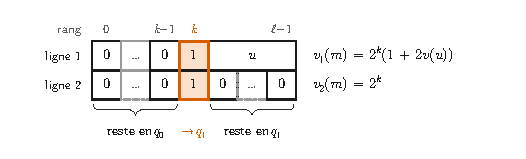
\includegraphics{figures/q4-forme-mots-a1.pdf}
\caption*{Figure 1 --- Forme d'un mot accepté par 𝒜₁ : k lettres nulles, la
colonne (1, 1) au rang k, puis une ligne 2 nulle et une ligne 1
quelconque u}
\end{figure}

\textbf{Étape 1 : \(\mathcal{L}({\mathcal{A}}_1)=R\).}

\begin{itemize}
\tightlist
\item
  \(R\subseteq\mathcal{L}({\mathcal{A}}_1)\) : le calcul \(q_0\xrightarrow{\binom00^k}q_0\xrightarrow{\binom11}q_1\xrightarrow{w}q_1\) existe et finit dans \(q_1\in F\).
\item
  \(\mathcal{L}({\mathcal{A}}_1)\subseteq R\) : soit \(q_{(0)}=q_0,\dots,q_{(\ell)}=q_1\) un calcul acceptant sur \(m=m_0\cdots m_{\ell-1}\). Il ne passe jamais par \(q_2\) : aucune transition n'en sort et \(q_2\notin F\).
\item
  Soit \(k\) le premier instant où \(q_{(k+1)}=q_1\). Pour \(t<k\), la transition \(q_0\xrightarrow{m_t}q_0\) impose \(m_t=\binom00\).
\item
  La transition \(q_0\xrightarrow{m_k}q_1\) impose \(m_k=\binom11\). Pour \(t>k\), \(q_1\xrightarrow{m_t}q_1\) impose \(m_t\in\{\binom00,\binom10\}\). Donc \(m\in R\).
\end{itemize}

\textbf{Étape 2 : \(R=E\).} Il n'existe pas de plus grande puissance de 2 divisant \(0\) : un mot avec \(v_1(m)=0\) n'est pas dans \(E\).

\begin{itemize}
\tightlist
\item
  \(R\subseteq E\) : soit \(m=\binom00^k\binom11w\) et \(u=\pi_1(w)\). Alors \(\pi_1(m)=0^k1u\) et \(\pi_2(m)=0^k10^{|w|}\), donc
\end{itemize}

\equationajustee{\begin{aligned}
v_2(m)&=2^k,\\
v_1(m)&=2^k+2^{k+1}v(u)=2^k\big(1+2v(u)\big).
\end{aligned}}

Le facteur \(1+2v(u)\) est impair : la plus grande puissance de 2 divisant \(v_1(m)\) est \(2^k=v_2(m)\).
- \(E\subseteq R\) : soit \(m\in E\) de longueur \(\ell\). Alors \(v_1(m)\ne0\) ; notons \(2^k\) la plus grande puissance de 2 qui le divise.
- Le bit de poids \(2^k\) de \(v_1(m)\) vaut 1 et ceux de poids inférieur sont nuls : \(\pi_1(m)=0^k1u\), avec \(k\le\ell-1\).
- Comme \(v_2(m)=2^k\), l'unicité de l'écriture binaire à longueur \(\ell\) donne \(\pi_2(m)=0^k10^{\ell-k-1}\).
- Les \(k\) premières lettres valent donc \(\binom00\), la suivante \(\binom11\), et les autres ont une ligne 2 nulle : \(m\in R\).

\equationajustee{\boxed{\mathcal{L}({\mathcal{A}}_1)=R=E}}

\hypertarget{question-5}{%
\subsection{Question 5}\label{question-5}}

Soit \(m\in\mathcal{L}({\mathcal{A}}_1)\). D'après Q4, \(v_2(m)=2^k\) et \(v_1(m)=2^k+2^{k+1}v(u)\) avec \(v(u)\in\mathbb{N}\). Donc

\equationajustee{v_1(m)-v_2(m)=\big(2\times v_2(m)\big)\,v(u),}

soit

\equationajustee{\boxed{v_1(m)\equiv v_2(m)\ [2\times v_2(m)]}}

\hypertarget{question-6}{%
\subsection{Question 6}\label{question-6}}

\equationajustee{\boxed{m\in\mathcal{L}({\mathcal{A}}_2)\iff v_1(m)>v_2(m)}}

(L'état courant est \(q_1\) exactement quand, à la dernière position où les deux lignes diffèrent, c'est-à-dire au bit de poids fort où les deux entiers diffèrent, la ligne 1 porte un 1.)

\hypertarget{question-7}{%
\subsection{Question 7}\label{question-7}}

Comme les lignes d'un mot ont la même longueur, \(v_i(m)=v_j(m)\iff\pi_i(m)=\pi_j(m)\).

On prend l'automate \(\mathcal{B}=(\Sigma_3,\allowbreak \{r_0,\allowbreak r_1,\allowbreak r_2\},\allowbreak r_0,\allowbreak \{r_0,\allowbreak r_1,\allowbreak r_2\},\allowbreak \delta)\), \textbf{tous les états finaux}, sans \(\varepsilon\)-transition, avec pour \(a=\langle a_1,a_2,a_3\rangle\) :

\begin{longtable}[]{@{}lll@{}}
\toprule\noalign{}
depuis & vers \(r_1\) si & vers \(r_2\) si \\
\midrule\noalign{}
\endhead
\bottomrule\noalign{}
\endlastfoot
\(r_0\) & \(a_1=a_3\) & \(a_2=a_3\) \\
\(r_1\) & \(a_1=a_3\) & jamais \\
\(r_2\) & jamais & \(a_2=a_3\) \\
\end{longtable}

L'état \(r_0\) accepte \(\varepsilon\) (où \(v_1=v_2=v_3=0\)).

Un mot non vide est accepté si toutes ses lettres vérifient \(a_1=a_3\) (chemin par \(r_1\)) ou toutes vérifient \(a_2=a_3\) (chemin par \(r_2\)).

\begin{figure}[H]
\centering
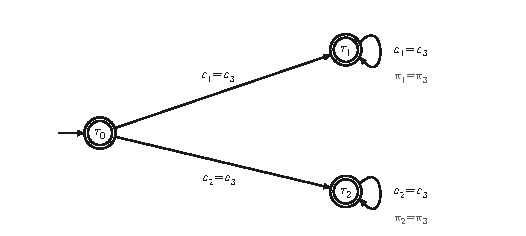
\includegraphics{figures/q7-automate-trois-etats.pdf}
\caption*{Figure 2 --- Automate à trois états pour L, tous finaux : r₁ suit π₁ =
π₃, r₂ suit π₂ = π₃}
\end{figure}

\hypertarget{question-8}{%
\subsection{Question 8}\label{question-8}}

\begin{lstlisting}[language=Caml]
let est_deterministe_complet a =
  let ok = ref true in
  for x = 0 to pow2 a.n - 1 do       (* x parcourt les 2^n lettres *)
    let lettre = decompose x a.n in
    for q = 0 to a.k - 1 do          (* tous les états, accessibles ou non *)
      match a.delta q lettre with
      | [_] -> ()                     (* exactement un successeur *)
      | _ -> ok := false
    done
  done;
  !ok
\end{lstlisting}

\textbf{Correction.} Par Q2 et Q3, \(x\mapsto\texttt{decompose x n}\) parcourt \(\Sigma_n\) une fois et une seule. La double boucle examine chaque couple \((q,a)\in Q\times\Sigma_n\), pour \textbf{tous} les états. \texttt{ok} reste vrai si et seulement si chaque liste \(\delta(q,a)\) a exactement un élément (listes sans doublon).

\textbf{Complexité.}

\begin{itemize}
\tightlist
\item
  Un appel à \texttt{delta} est compté \(O(n)\) (il reçoit une lettre de taille \(n\)).
\item
  Le filtrage \texttt{{[}\_{]}} est en \(O(1)\) : il ne parcourt pas la liste, contrairement à \texttt{List.length}.
\item
  \texttt{pow2\ a.n} est évalué une fois, en \(O(\log n)\).
\item
  Pour chacune des \(2^n=|\Sigma_n|\) lettres : \texttt{decompose} en \(O(n)\), puis \(|Q|\) appels en \(O(n)\).
\end{itemize}

Total :

\equationajustee{O(\log n)+|\Sigma_n|\big(O(n)+|Q|\,O(n)\big)=\boxed{O\big(n\times|Q|\times|\Sigma_n|\big)}}

\hypertarget{question-9}{%
\subsection{Question 9}\label{question-9}}

Soit \(\mathcal{A}=(\Sigma,Q,q_0,F,\delta)\). L'automate des parties est \({\mathcal{A}}^d=\big(\Sigma,\allowbreak \ \mathcal{P}(Q),\allowbreak \ \{q_0\},\allowbreak \ F^d,\allowbreak \ \delta^d\big)\), avec :

\equationajustee{\begin{aligned}{}&\text{\text{états} : } \mathcal{P}(Q), \qquad \text{\text{état} initial : } \{q_0\},\\
&\delta^d(S,a)=\Big\{\bigcup_{q\in S}\delta(q,a)\Big\} \quad\text{pour } S\subseteq Q,\ a\in\Sigma,\\
&F^d=\{S\subseteq Q \mid S\cap F\ne\emptyset\}.
\end{aligned}}

Chaque \(\delta^d(S,a)\) est un singleton : \({\mathcal{A}}^d\) est déterministe complet (\(\emptyset\) est un état puits).

Par récurrence sur \(|m|\), l'unique état atteint depuis \(S\) en lisant \(m\) est \(\bigcup_{q\in S}\widehat\delta(q,m)\).

C'est vrai pour \(\varepsilon\) ; pour \(m=m'a\), on applique \(\delta^d\) à \(\bigcup_{q\in S}\widehat\delta(q,m')\). Donc

\equationajustee{m\in\mathcal{L}({\mathcal{A}}^d)\iff\widehat\delta(q_0,m)\cap F\ne\emptyset\iff m\in\mathcal{L}(\mathcal{A}).}

\hypertarget{question-10}{%
\subsection{Question 10}\label{question-10}}

\begin{lstlisting}[language=Caml]
let union etats a lettre =
  let t = Array.make a.k 0 in
  for q = 0 to a.k - 1 do
    if etats.(q) = 1 then
      List.iter (fun i -> t.(i) <- 1) (a.delta q lettre)
  done;
  t
\end{lstlisting}

\texttt{t.(i)} passe à 1 exactement quand \(i\in\delta(q,\texttt{lettre})\) pour un \(q\) tel que \texttt{etats.(q)\ =\ 1}, et reste à 0 sinon. Le tableau est neuf, initialisé à 0, et \texttt{etats} n'est pas modifié. Les transitions ne sont parcourues qu'une fois.

\hypertarget{question-11}{%
\subsection{Question 11}\label{question-11}}

Une partie de \([\![0,k-1]\!]\) est codée par son vecteur caractéristique, élément de \(\Sigma_k\), donc par un entier de \([\![0,2^k-1]\!]\) (Q2).

Le singleton \(\{0\}\) a pour code \(1\).

Comme l'état initial doit porter le numéro \(0\), on numérote les états par la transposition qui échange les codes \(0\) et \(1\).

\begin{lstlisting}[language=Caml]
(* involution de [0, 2^k - 1] : échange 0 et 1 *)
let echange x = if x = 0 then 1 else if x = 1 then 0 else x

let determinise a =
  let kd = pow2 a.k in
  let ens i = decompose (echange i) a.k in   (* numéro -> partie *)
  let code t =                               (* partie -> numéro *)
    let x = ref 0 and p = ref 1 in
    for q = 0 to a.k - 1 do
      if t.(q) = 1 then x := !x + !p;
      p := 2 * !p
    done;
    echange !x
  in
  let finaux = Array.make kd false in
  for i = 0 to kd - 1 do
    let s = ens i in
    for q = 0 to a.k - 1 do
      if s.(q) = 1 && a.finaux.(q) then finaux.(i) <- true
    done
  done;
  { k = kd; n = a.n; finaux = finaux;
    delta = (fun i lettre -> [ code (union (ens i) a lettre) ]) }
\end{lstlisting}

\textbf{Correction.} \texttt{ens} est une bijection de \([\![0,2^k-1]\!]\) sur \(\mathcal{P}([\![0,k-1]\!])\) (composée de deux bijections) et \texttt{code} est sa réciproque. L'état \(0\) code \(\{0\}=\{q_0\}\).

\texttt{delta} renvoie le singleton du code de \(\bigcup_{q\in S}\delta(q,a)\) (Q10), et \texttt{finaux.(i)} est vrai si et seulement si la partie codée rencontre \(F\). C'est l'automate \({\mathcal{A}}^d\) de Q9 : déterministe complet et équivalent à \texttt{a}.

\hypertarget{question-12}{%
\subsection{Question 12}\label{question-12}}

\begin{lstlisting}[language=Caml]
let complementaire a =
  let d = if est_deterministe_complet a then a else determinise a in
  { k = d.k; n = d.n; finaux = Array.map not d.finaux; delta = d.delta }
\end{lstlisting}

L'automate \(d\) est déterministe complet et \(\mathcal{L}(d)=\mathcal{L}(a)\) (Q11).

Tout mot \(m\) a un unique calcul dans \(d\), d'état d'arrivée \(p(m)\).

Le mot \(m\) est accepté par le résultat si et seulement si \(p(m)\notin F_d\), c'est-à-dire \(m\notin\mathcal{L}(a)\).

\textbf{On obtient le complémentaire dans \(\Sigma_n^*\).} Sans complétude, l'échange des finaux est faux : un mot sans calcul serait rejeté par les deux automates.

\hypertarget{question-13}{%
\subsection{Question 13}\label{question-13}}

On pose \({\mathcal{A}}_\cap=\big(\Sigma_n,\allowbreak \ Q_1\times Q_2,\allowbreak \ (q_1,\allowbreak q_2),\allowbreak \ F_1\times F_2,\allowbreak \ \delta\big)\), avec :

\equationajustee{\begin{aligned}{}&\text{\text{état} initial : } (q_1,q_2), \qquad \text{\text{états} finaux : } F_1\times F_2,\\
&\delta\big((p,q),a\big)=\delta_1(p,a)\times\delta_2(q,a)\quad\text{pour }(p,q)\in Q_1\times Q_2,\ a\in\Sigma_n.
\end{aligned}}

Par récurrence sur \(|m|\) :

\equationajustee{\widehat\delta\big((q_1,q_2),m\big)=\widehat\delta_1(q_1,m)\times\widehat\delta_2(q_2,m).}

C'est vrai pour \(\varepsilon\). Pour \(m=m'a\), l'union des \(\delta_1(p',a)\times\delta_2(q',a)\) sur un produit \(P_1\times P_2\) est le produit des unions.

Or \((R_1\times R_2)\cap(F_1\times F_2)\ne\emptyset\) si et seulement si \(R_1\cap F_1\ne\emptyset\) et \(R_2\cap F_2\ne\emptyset\). Donc \(\mathcal{L}({\mathcal{A}}_\cap)=\mathcal{L}({\mathcal{A}}_1)\cap\mathcal{L}({\mathcal{A}}_2)\). Aucune hypothèse de déterminisme n'est nécessaire.

\hypertarget{opuxe9rations-arithmuxe9tiques}{%
\section{3. Opérations arithmétiques}\label{opuxe9rations-arithmuxe9tiques}}

\hypertarget{question-14}{%
\subsection{Question 14}\label{question-14}}

Deux états : \(r_0\) (retenue 0, initial et \textbf{seul final}) et \(r_1\) (retenue 1). La transition \(r_c\xrightarrow{\langle\alpha,\beta,\sigma\rangle}r_{c'}\) existe si et seulement si \(\alpha+\beta+c=\sigma+2c'\) :

\begin{longtable}[]{@{}
  >{\raggedright\arraybackslash}p{(\columnwidth - 4\tabcolsep) * \real{0.0859}}
  >{\raggedright\arraybackslash}p{(\columnwidth - 4\tabcolsep) * \real{0.4421}}
  >{\raggedright\arraybackslash}p{(\columnwidth - 4\tabcolsep) * \real{0.4421}}@{}}
\toprule\noalign{}
\begin{minipage}[b]{\linewidth}\raggedright
depuis
\end{minipage} & \begin{minipage}[b]{\linewidth}\raggedright
lettre \(\to r_0\)
\end{minipage} & \begin{minipage}[b]{\linewidth}\raggedright
lettre \(\to r_1\)
\end{minipage} \\
\midrule\noalign{}
\endhead
\bottomrule\noalign{}
\endlastfoot
\(r_0\) & \(\langle0,\allowbreak 0,\allowbreak 0\rangle,\allowbreak \ \langle1,\allowbreak 0,\allowbreak 1\rangle,\allowbreak \ \langle0,\allowbreak 1,\allowbreak 1\rangle\) & \(\langle1,1,0\rangle\) \\
\(r_1\) & \(\langle0,0,1\rangle\) & \(\langle1,\allowbreak 0,\allowbreak 0\rangle,\allowbreak \ \langle0,\allowbreak 1,\allowbreak 0\rangle,\allowbreak \ \langle1,\allowbreak 1,\allowbreak 1\rangle\) \\
\end{longtable}

Les autres couples (état, lettre) n'ont pas de transition.

\begin{figure}[H]
\centering
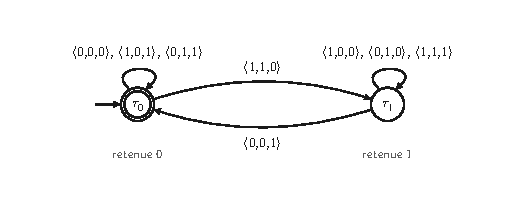
\includegraphics{figures/q14-automate-retenue.pdf}
\caption*{Figure 3 --- Automate de l'addition : l'état est la retenue, seul r₀ est
final}
\end{figure}

\hypertarget{question-15}{%
\subsection{Question 15}\label{question-15}}

Soit \(m=m_0\cdots m_{\ell-1}\) avec \(m_t=\langle\alpha_t,\beta_t,\sigma_t\rangle\). Pour \(0\le t\le\ell\), on pose

\equationajustee{A_t=\sum_{j<t}2^j\alpha_j,}

et \(B_t\), \(S_t\) de même. Ce sont les valeurs des préfixes, dans \([\![0,2^t-1]\!]\), et \(A_\ell=v_1(m)\), \(B_\ell=v_2(m)\), \(S_\ell=v_3(m)\).

\textbf{Propriété \(\mathcal{P}(t)\)} : il existe un calcul depuis \(r_0\) sur \(m_0\cdots m_{t-1}\) si et seulement s'il existe \(c\in\{0,1\}\) tel que \(A_t+B_t=S_t+2^tc\).

Ce \(c\) est alors unique, et le calcul (unique, l'automate étant déterministe) arrive en \(r_c\).

\(\mathcal{P}(0)\) : calcul vide en \(r_0\), et \(0=0+2^0c\) force \(c=0\). Supposons \(\mathcal{P}(t)\), et notons \(m_t=\langle\alpha,\beta,\sigma\rangle\).

\begin{itemize}
\item
  (\(\Rightarrow\)) Un calcul sur \(t+1\) lettres passe, après \(t\) lettres, par \(r_c\) avec \(A_t+B_t=S_t+2^tc\).

  Il emprunte ensuite \(r_c\xrightarrow{m_t}r_{c'}\), donc \(\alpha+\beta+c=\sigma+2c'\). Alors
\end{itemize}

\equationajustee{\begin{aligned}
A_{t+1}+B_{t+1}&=S_t+2^t(c+\alpha+\beta)\\
&=S_t+2^t(\sigma+2c')\\
&=S_{t+1}+2^{t+1}c'.
\end{aligned}}

\begin{itemize}
\tightlist
\item
  (\(\Leftarrow\)) Supposons \(A_{t+1}+B_{t+1}=S_{t+1}+2^{t+1}c'\) avec \(c'\in\{0,1\}\). Alors \(A_t+B_t=S_t+2^tc\) avec \(c=\sigma-\alpha-\beta+2c'\in\mathbb{Z}\).
\item
  Comme \(-(2^t-1)\le A_t+B_t-S_t\le2(2^t-1)\), on a \(-2^t<2^tc<2^{t+1}\), donc \(c\in\{0,1\}\).
\item
  Par \(\mathcal{P}(t)\), le calcul arrive en \(r_c\), et \(\alpha+\beta+c=\sigma+2c'\) est exactement la condition d'existence de \(r_c\xrightarrow{m_t}r_{c'}\).
\item
  Unicité : \(c'=(A_{t+1}+B_{t+1}-S_{t+1})/2^{t+1}\).
\end{itemize}

Conclusion avec \(t=\ell\) : \(m\) est accepté si et seulement si le calcul existe et arrive en \(r_0\), si et seulement si \(v_1(m)+v_2(m)=v_3(m)+2^\ell\cdot0\). \textbf{L'automate reconnaît \(L_+\).}

\hypertarget{question-16}{%
\subsection{Question 16}\label{question-16}}

\textbf{Non, \(L_\times\) n'est pas reconnaissable.} Supposons-le reconnu par un automate à \(N\) états et posons \(p=N\). Soit \(m\in\Sigma_3^*\) de longueur \(2p+1\) avec

\equationajustee{\begin{aligned}
\pi_1(m)&=0^p\,1\,0^p,\\
\pi_2(m)&=0^p\,1\,0^p,\\
\pi_3(m)&=0^{2p}\,1.
\end{aligned}}

Alors \(v_1(m)=v_2(m)=2^p\) et \(v_3(m)=2^{2p}\) : \(m\in L_\times\).

Le lemme de l'étoile donne \(m=xyz\) avec \(|xy|\le p\), \(y\ne\varepsilon\) et \(xy^iz\in L_\times\) pour tout \(i\).

Les \(p\) premières lettres de \(m\) valent \(\mathbf{0}\), donc \(y={\mathbf{0}}^\lambda\) avec \(\lambda\ge1\).

Dans \(xy^2z\), on a inséré \(\lambda\) colonnes nulles avant toutes les positions des 1 :

\equationajustee{\begin{aligned}
v_1(xy^2z)=v_2(xy^2z)&=2^{p+\lambda},\\
v_1(xy^2z)\times v_2(xy^2z)&=2^{2p+2\lambda},\\
v_3(xy^2z)&=2^{2p+\lambda}\ne2^{2p+2\lambda}.
\end{aligned}}

Donc \(xy^2z\notin L_\times\) : contradiction.

\begin{figure}[H]
\centering
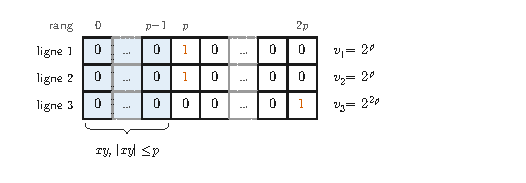
\includegraphics{figures/q16-mot-pompage.pdf}
\caption*{Figure 4 --- Mot pompé : les p premières colonnes sont nulles, donc le
facteur y aussi}
\end{figure}

\hypertarget{arithmuxe9tique-de-presburger}{%
\section{4. Arithmétique de Presburger}\label{arithmuxe9tique-de-presburger}}

\hypertarget{question-17}{%
\subsection{Question 17}\label{question-17}}

\equationajustee{\boxed{{\mathrm{div}}_2(x):=\exists y.\ x=y+y}}

Sous l'assignation \(x\mapsto k\), la formule est vraie si et seulement s'il existe \(j\in\mathbb{N}\) avec \(k=j+j=2j\), c'est-à-dire si \(2\mid k\).

\hypertarget{question-18}{%
\subsection{Question 18}\label{question-18}}

Aucune constante n'est un terme : on caractérise \(0\), puis \(1\).

\begin{itemize}
\tightlist
\item
  \(\mathrm{zero}(z):=(z=z+z)\) : dans \(\mathbb{N}\), \(z=2z\iff z=0\).
\item
  On pose
\end{itemize}

\equationajustee{\begin{aligned}
\mathrm{un}(u):=\ &\neg(u=u+u)\\
&\wedge\neg\exists s.\exists t.\big(\neg(s=s+s)\wedge\neg(t=t+t)\wedge u=s+t\big).
\end{aligned}}

Elle dit que \(u\) est non nul et n'est pas somme de deux entiers non nuls. Si \(u=1\), toute écriture \(1=s+t\) a un terme nul.

Si \(u\ge2\), l'écriture \(u=1+(u-1)\) a deux termes non nuls. Le cas \(u=0\) est exclu par le premier conjoint.

Donc \(\mathrm{un}(u)\) est vraie si et seulement si \(u=1\).

\equationajustee{\boxed{\begin{aligned}
f_0(x)&:=\big(x=x+x\big),\\
f_n(x)&:=\exists u.\Big(\mathrm{un}(u)\wedge x=\underbrace{u+u+\cdots+u}_{n\text{ termes}}\Big)\quad(n\ge1).
\end{aligned}}}

Pour \(n\ge1\), la formule est vraie si et seulement s'il existe \(u\) valant \(1\) avec \(a(x)=n\,u\), c'est-à-dire \(a(x)=n\).

Les variables \(u,s,t\) sont distinctes de \(x\) et liées ; \(x\) est la seule variable libre.

\hypertarget{question-19}{%
\subsection{Question 19}\label{question-19}}

\textbf{Stratégie.} Induction structurelle sur l'ensemble des formules de Presburger. Pour une formule \(\varphi\), la propriété démontrée est :

\begin{quote}

\(\mathcal{P}(\varphi)\) : on sait construire une formule \(S(\varphi)\) sous forme simple, de mêmes variables libres que \(\varphi\) et équivalente à \(\varphi\).

\end{quote}

Les variables introduites sont \textbf{fraîches} (\(\mathcal{V}\) est infini).

Le cas de base (les atomes) assure la condition (iii) ; les cas inductifs traitent \(\neg\), \(\wedge\), \(\exists\), puis éliminent \(\vee\), \(\to\) et \(\forall\).

\textbf{Cas de base : atomes.} Tout terme s'écrit \(y_1+\cdots+y_p\) (\(p\ge1\), \(y_r\) variables), par induction sur les termes et associativité.

\emph{Lemme.} Si \(z\) n'apparaît ni dans le terme \(t\) ni dans \(\psi\), alors \(\exists z.(z=t\wedge\psi)\) est équivalente à \(\psi[t/z]\).

En effet, pour toute assignation, le seul témoin possible est la valeur de \(t\), qui est dans \(\mathbb{N}\).

Considérons l'atome \(y_1+\cdots+y_p=y'_1+\cdots+y'_q\). On pose \(z_1:=y_1\) et \(z'_1:=y'_1\), et on prend des variables fraîches \(z_2,\dots,z_p,z'_2,\dots,z'_q\). On définit

\equationajustee{\begin{aligned}
C&:=\bigwedge_{r=2}^p \big(z_r=z_{r-1}+y_r\big),\\
C'&:=\bigwedge_{s=2}^q \big(z'_s=z'_{s-1}+y'_s\big),\\
S(t_1=t_2)&:=\exists z_2\cdots\exists z_p\,\exists z'_2\cdots\exists z'_q.\big(C\wedge C'\wedge z_p=z'_q\big).
\end{aligned}}

Chaque atome a la forme « variable \(=\) variable » ou « variable \(=\) variable \(+\) variable » : (iii) est respectée.

Il n'y a ni \(\vee\), ni \(\to\), ni \(\forall\). En appliquant le lemme de l'intérieur vers l'extérieur, on retrouve l'atome initial ; les \(z\) sont liées, donc les variables libres sont inchangées.

\textbf{Cas inductifs.} Par hypothèse d'induction, \(S(\varphi)\), \(S(\varphi_1)\) et \(S(\varphi_2)\) sont sous forme simple et équivalentes à \(\varphi\), \(\varphi_1\), \(\varphi_2\). On pose :

\equationajustee{\begin{aligned}
S(\neg\varphi)&:=\neg S(\varphi),\\
S(\varphi_1\wedge\varphi_2)&:=S(\varphi_1)\wedge S(\varphi_2),\\
S(\exists x.\varphi)&:=\exists x.S(\varphi),\\
S(\varphi_1\vee\varphi_2)&:=\neg\big(\neg S(\varphi_1)\wedge\neg S(\varphi_2)\big),\\
S(\varphi_1\to\varphi_2)&:=\neg\big(S(\varphi_1)\wedge\neg S(\varphi_2)\big),\\
S(\forall x.\varphi)&:=\neg\exists x.\neg S(\varphi).
\end{aligned}}

\begin{itemize}
\tightlist
\item
  Les trois dernières lignes reposent sur des équivalences vraies sous toute assignation : De Morgan, \(A\to B\equiv\neg(A\wedge\neg B)\) et \(\forall x.A\equiv\neg\exists x.\neg A\).
\item
  La valeur de vérité de \(\neg\), \(\wedge\), \(\exists\) ne dépend de leurs sous-formules que par leurs valeurs de vérité : remplacer \(\varphi_r\) par \(S(\varphi_r)\), équivalente, conserve l'équivalence.
\item
  Les propriétés (i), (ii), (iii) sont stables par \(\neg\), \(\wedge\), \(\exists\), et les variables libres sont conservées.
\item
  \(S(\exists x.\varphi)\) est bien formée : les variables fraîches diffèrent de \(x\), et \(S\) ne quantifie que les variables déjà quantifiées dans \(\varphi\).
\end{itemize}

\textbf{Toute formule de Presburger est équivalente à une formule sous forme simple.}

\hypertarget{question-20}{%
\subsection{Question 20}\label{question-20}}

On note \(A=\varphi(x)\), \(B=\psi(y)\) et \(\Gamma=\{A\vee B,\ \neg A\}\). Aucune règle de quantificateur n'intervient.

\equationajustee{\dfrac{\dfrac{\dfrac{\Gamma\vdash A\vee B\ (\mathrm{ax})\qquad\dfrac{\dfrac{\Gamma,A\vdash\neg A\ (\mathrm{ax})\qquad\Gamma,A\vdash A\ (\mathrm{ax})}{\Gamma,A\vdash\bot}\,\neg e}{\Gamma,A\vdash B}\,\bot\qquad\Gamma,B\vdash B\ (\mathrm{ax})}{\Gamma\vdash B}\,\vee e}{A\vee B\vdash\neg A\to B}\,\to i}{\vdash(A\vee B)\to(\neg A\to B)}\,\to i}

\hypertarget{question-21}{%
\subsection{Question 21}\label{question-21}}

\equationajustee{\boxed{\begin{aligned}
T:=\ &\forall x.\forall y.\forall z.\\
&\Big(\big(x=y\wedge y=z\big)\to x=z\Big)
\end{aligned}}}

Soit \(\Delta=\{y=z,\ x=y\}\). L'arbre est écrit ligne par ligne, de la feuille (1) à la racine (7) ; chaque ligne est la conclusion de la règle indiquée appliquée à la ligne précédente.

\equationajustee{\begin{array}{lll}
(1) & \Delta\vdash y=z & \mathrm{ax}\\
(2) & \Delta\vdash x=z & {\mathrm{sub}}_=\ \text{sur }(1)\\
(3) & x=y\wedge y=z\vdash x=z & \mathrm{cut}\ \text{sur }(2)\\
(4) & \vdash(x=y\wedge y=z)\to x=z & {\to}i\ \text{sur }(3)\\
(5) & \vdash\forall z.\big((x=y\wedge y=z)\to x=z\big) & \forall i\ \text{sur }(4)\\
(6) & \vdash\forall y.\forall z.\big((x=y\wedge y=z)\to x=z\big) & \forall i\ \text{sur }(5)\\
(7) & \vdash T & \forall i\ \text{sur }(6)
\end{array}}

\begin{itemize}
\item
  Ligne (2) : instance de \({\mathrm{sub}}_=\) avec la variable \(x\), le terme \(y\), le contexte \(\{y=z\}\) et la formule \(x=z\).

  La prémisse demandée est \((x=z)[y/x]\), c'est-à-dire \(y=z\) : c'est la ligne (1).
\item
  Ligne (3) : la règle cut transforme les deux hypothèses \(x=y\), \(y=z\) en la conjonction.
\item
  Lignes (5) à (7) : les trois \(\forall i\) sont licites, car le contexte est vide (\(z,y,x\notin FV(\emptyset)\)).
\end{itemize}

\hypertarget{question-22}{%
\subsection{Question 22}\label{question-22}}

Soit \(\Delta=\{x=y+a,\ y=z+b\}\) et

\equationajustee{\begin{aligned}
\Phi:=\ &\big(\exists a.\exists b.(x=y+a\wedge y=z+b)\big)\\
&\to\exists c.\,x=z+c.
\end{aligned}}

Seule l'associativité est permise : le témoin est \(c:=b+a\) (et non \(a+b\)). L'arbre est écrit ligne par ligne, de la feuille (1) à la racine (11).

\equationajustee{\begin{array}{lll}
(1) & \Delta\vdash z+b+a=z+b+a & {\mathrm{ax}}_=\\
(2) & \Delta\vdash y+a=z+b+a & {\mathrm{sub}}_=\ \text{sur }(1)\\
(3) & \Delta\vdash x=z+b+a & {\mathrm{sub}}_=\ \text{sur }(2)\\
(4) & \Delta\vdash \exists c.\,x=z+c & \exists i\ \text{sur }(3)\\
(5) & x=y+a\wedge y=z+b\vdash \exists c.\,x=z+c & \mathrm{cut}\ \text{sur }(4)\\
(6) & \exists b.(x=y+a\wedge y=z+b)\vdash \exists c.\,x=z+c & \exists' e\ \text{sur }(5)\\
(7) & \exists a.\exists b.(x=y+a\wedge y=z+b)\vdash \exists c.\,x=z+c & \exists' e\ \text{sur }(6)\\
(8) & \vdash\Phi & {\to}i\ \text{sur }(7)\\
(9) & \vdash\forall z.\,\Phi & \forall i\ \text{sur }(8)\\
(10) & \vdash\forall y.\forall z.\,\Phi & \forall i\ \text{sur }(9)\\
(11) & \vdash\forall x.\forall y.\forall z.\,\Phi & \forall i\ \text{sur }(10)
\end{array}}

Instances et conditions de bord :

\begin{itemize}
\item
  Ligne (2) : \({\mathrm{sub}}_=\) avec la variable \(y\), le terme \(z+b\), le contexte \(\{x=y+a\}\) et la formule \(y+a=z+b+a\).

  La substitution donne \((z+b)+a=z+b+a\), instance de \({\mathrm{ax}}_=\) à l'associativité près.
\item
  Ligne (3) : \({\mathrm{sub}}_=\) avec la variable \(x\), le terme \(y+a\), le contexte \(\{y=z+b\}\) et la formule \(x=z+b+a\). La substitution donne \(y+a=z+b+a\) : c'est la ligne (2).
\item
  Ligne (4) : \(\exists i\) avec le terme \(b+a\). La formule \((x=z+c)[b+a/c]\) est \(x=z+(b+a)\), c'est-à-dire \(x=z+b+a\) par associativité.
\item
  Lignes (6) et (7) : pour \(\exists' e\) sur \(b\) puis sur \(a\), le contexte restant est vide, et \(FV(\exists c.\,x=z+c)=\{x,z\}\) ne contient ni \(b\) ni \(a\).
\item
  Lignes (9) à (11) : les \(\forall i\) sont licites, car le contexte est vide.
\end{itemize}

\hypertarget{retour-sur-les-automates}{%
\section{5. Retour sur les automates}\label{retour-sur-les-automates}}

\hypertarget{question-23}{%
\subsection{Question 23}\label{question-23}}

Soit \(\varphi\) une CNF sur les variables propositionnelles \(p_1,\dots,p_N\). On prend \(N\) variables de Presburger distinctes \(u_1,\dots,u_N\).

On remplace chaque occurrence de \(p_i\) par la formule de Presburger \(T_i:=\neg(u_i=u_i+u_i)\) (« \(u_i\ne0\) »), en conservant \(\neg\), \(\wedge\), \(\vee\).

On obtient une formule de Presburger \(\mathrm{tr}(\varphi)\), puis

\equationajustee{\boxed{\Psi:=\exists u_1.\exists u_2\cdots\exists u_N.\ \mathrm{tr}(\varphi)}}

formule close, donc instance de Tautologie-Presburger.

\textbf{Correction.} À tout \((n_1,\dots,n_N)\in{\mathbb{N}}^N\), on associe la valuation \(\theta(p_i)=(n_i\ne0)\). Toute valuation est obtenue ainsi (prendre \(n_i\in\{0,1\}\)).

Par induction sur la formule, \(\mathrm{tr}(\alpha)\) est vraie sous l'assignation \(u_i\mapsto n_i\) si et seulement si \(\alpha\) est vraie sous \(\theta\).

Donc \(\Psi\) est vraie si et seulement si \(\varphi\) est satisfiable.

\textbf{Coût.} Chaque littéral est remplacé par une formule de taille constante, et on ajoute \(N\) quantificateurs : \(|\Psi|=O(|\varphi|)\), construite par un parcours linéaire. \textbf{Sat-Cnf se réduit polynomialement à Tautologie-Presburger} (qui est donc NP-difficile).

\hypertarget{question-24}{%
\subsection{Question 24}\label{question-24}}

Ici \(n=3\) et \(L=\{\varepsilon,\allowbreak \ \langle0,\allowbreak 1,\allowbreak 1\rangle,\allowbreak \ \langle0,\allowbreak 0,\allowbreak 0\rangle\langle1,\allowbreak 1,\allowbreak 1\rangle\}\). Un mot de \(L_{\exists2}\) a la longueur et les lignes 1 et 3 d'un mot de \(L\), la ligne 2 étant quelconque. On énumère donc, pour chaque mot de \(L\), les deux choix de bit en ligne 2 à chaque position :

\equationajustee{\boxed{\begin{aligned}
L_{\exists2}=\big\{&\varepsilon,\\
&\langle0,0,1\rangle,\ \langle0,1,1\rangle,\\
&\langle0,0,0\rangle\langle1,0,1\rangle,\ \langle0,0,0\rangle\langle1,1,1\rangle,\\
&\langle0,1,0\rangle\langle1,0,1\rangle,\ \langle0,1,0\rangle\langle1,1,1\rangle\big\}
\end{aligned}}}

soit \(1+2+4=7\) mots.

\hypertarget{question-25}{%
\subsection{Question 25}\label{question-25}}

On garde les états, l'état initial et les finaux. On remplace \(\delta\) par

\equationajustee{\delta'(q,a)=\delta(q,a[i\leftarrow0])\cup\delta(q,a[i\leftarrow1]),}

où \(a[i\leftarrow\beta]\) est la lettre \(a\) dont la composante \(i\) vaut \(\beta\).

\begin{lstlisting}[language=Caml]
let automate_existe a i =
  let delta' q lettre =
    let l0 = Array.copy lettre and l1 = Array.copy lettre in
    l0.(i - 1) <- 0;          (* ligne i = indice i-1 *)
    l1.(i - 1) <- 1;
    List.sort_uniq compare (a.delta q l0 @ a.delta q l1)
  in
  { k = a.k; n = a.n; finaux = a.finaux; delta = delta' }
\end{lstlisting}

\textbf{Correction.}

\begin{itemize}
\item
  Si \(m\) a un calcul acceptant dans le nouvel automate, chaque pas \(q_{(t)}\to q_{(t+1)}\) provient d'une lettre \(w_t=m_t[i\leftarrow\beta_t]\).

  Le mot \(w=w_0\cdots w_{\ell-1}\) est accepté par \(\mathcal{A}\) et coïncide avec \(m\) hors de la ligne \(i\).
\item
  Réciproquement, soit \(w\in\mathcal{L}(\mathcal{A})\) qui coïncide avec \(m\) hors de la ligne \(i\).

  Alors \(|w|=|m|\), \(w_t=m_t[i\leftarrow\pi_i(w)_t]\) et \(\delta(q,w_t)\subseteq\delta'(q,m_t)\) : le calcul acceptant de \(w\) est un calcul acceptant de \(m\).
\item
  La lettre reçue n'est pas modifiée (pas d'effet de bord) : on travaille sur deux copies.
\end{itemize}

\hypertarget{question-26}{%
\subsection{Question 26}\label{question-26}}

On fixe \(n\) (plus grand indice de variable) pendant tout le calcul : tous les automates sont sur \(\Sigma_n\), la ligne \(i\) portant la variable \(x_i\). On construit l'automate de \(\varphi\) \textbf{récursivement sur la structure de la formule} :

\begin{itemize}
\tightlist
\item
  \textbf{Atome \(x_i=x_j\)} : \texttt{automate\_egalite\ n\ i\ j}.
\item
  \textbf{Atome \(x_i=x_j+x_k\)} : \texttt{automate\_somme\ n\ j\ k\ i} (cette fonction reconnaît \(v_j+v_k=v_i\) ; elle suppose \(n\ge3\)).
\item
  \textbf{\(\neg\psi\)} : complémentaire (Q12) de l'automate de \(\psi\).
\item
  \textbf{\(\psi_1\wedge\psi_2\)} : intersection des deux automates.
\item
  \textbf{\(\exists x_i.\psi\)} : on rend la ligne \(i\) libre par \texttt{automate\_existe} (Q25) sur l'automate de \(\psi\), puis on applique \texttt{sans\_zero}.
\end{itemize}

\textbf{Pourquoi \texttt{sans\_zero}.} La projection ne change pas la longueur du mot : elle ne permet pour \(x_i\) que des valeurs codables sur \(|m|\) bits, alors que \(\exists x_i\) porte sur tout \(\mathbb{N}\).

Ajouter des lettres \(\mathbf{0}\) à droite ne change aucune valeur \(v_k\) (bits de poids fort nuls). Un mot \(m\) doit donc être accepté dès qu'un allongement \(m{\mathbf{0}}^j\) laisse la place au témoin. C'est exactement ce que fait \texttt{sans\_zero}, qui reconnaît \(\{m\mid\exists j\ge0,\allowbreak \ m{\mathbf{0}}^j\in\mathcal{L}(\mathcal{A})\}\).

Par exemple, avec \(n=3\) et \(\exists x_1.\,x_1=x_2+x_2\), le mot de longueur 1 tel que \(v_2=1\) doit être accepté (témoin \(x_1=2\)). Or aucun mot de longueur 1 ne code \(2\) sur la ligne 1.

\hypertarget{question-27}{%
\subsection{Question 27}\label{question-27}}

On traite \(\varphi(x_2):=\neg\exists x_1.\neg(x_1=x_2)\) avec \(n=2\), en suivant le code (Q11, Q12, Q25). Pour la feuille, on suppose que \texttt{automate\_egalite\ 2\ 1\ 2} renvoie l'automate à un état \(s\), initial et final, bouclant sur \(\binom00\) et \(\binom11\), sans autre transition.

\textbf{Étape 1} --- \({\mathcal{B}}_1\) reconnaît \(\{m\mid v_1(m)=v_2(m)\}\) (toutes les lettres valent \(\binom00\) ou \(\binom11\)).

\textbf{Étape 2} --- \(\neg(x_1=x_2)\). \({\mathcal{B}}_1\) n'est pas complet : on déterminise (\(k=1\), donc \(2\) états).

L'état \(0\) est \(\{s\}\), l'état \(1\) est \(\emptyset\) :

\begin{longtable}[]{@{}
  >{\raggedright\arraybackslash}p{(\columnwidth - 6\tabcolsep) * \real{0.2500}}
  >{\raggedright\arraybackslash}p{(\columnwidth - 6\tabcolsep) * \real{0.2500}}
  >{\raggedright\arraybackslash}p{(\columnwidth - 6\tabcolsep) * \real{0.2500}}
  >{\raggedright\arraybackslash}p{(\columnwidth - 6\tabcolsep) * \real{0.2500}}@{}}
\toprule\noalign{}
\begin{minipage}[b]{\linewidth}\raggedright
état
\end{minipage} & \begin{minipage}[b]{\linewidth}\raggedright
\(\binom00,\binom11\)
\end{minipage} & \begin{minipage}[b]{\linewidth}\raggedright
\(\binom01,\binom10\)
\end{minipage} & \begin{minipage}[b]{\linewidth}\raggedright
final après échange
\end{minipage} \\
\midrule\noalign{}
\endhead
\bottomrule\noalign{}
\endlastfoot
\(0=\{s\}\) & \(0\) & \(1\) & non \\
\(1=\emptyset\) & \(1\) & \(1\) & oui \\
\end{longtable}

\({\mathcal{B}}_2\) reconnaît \(\{m\mid v_1(m)\ne v_2(m)\}\).

\textbf{Étape 3} --- \texttt{automate\_existe} sur la ligne 1. Depuis \(0\), une lettre de ligne 2 égale à \(b\) donne les deux lettres \(\binom0b\) et \(\binom1b\), l'une vers \(0\), l'autre vers \(1\).

\begin{itemize}
\tightlist
\item
  Pour toute lettre \(a\) : \(\delta_3(0,a)=\{0,1\}\) et \(\delta_3(1,a)=\{1\}\).
\item
  Finaux : \(\{1\}\). \({\mathcal{B}}_3\) reconnaît \(\Sigma_2^*\setminus\{\varepsilon\}\).
\end{itemize}

\textbf{Étape 4} --- \texttt{sans\_zero}. Depuis \(0\), la lettre \(\binom00\) mène en \(1\), final : \(0\) devient final. \({\mathcal{B}}_4\) a les mêmes transitions et \textbf{tous ses états finaux} ; il reconnaît \(\Sigma_2^*\).

C'est bien \(L_{\exists x_1.\neg(x_1=x_2)}\) : pour tout \(x_2\), \(x_1=x_2+1\) convient, y compris pour \(\varepsilon\).

\textbf{Étape 5} --- négation extérieure. \({\mathcal{B}}_4\) n'est pas déterministe (\(\delta_4(0,a)=\{0,1\}\)) : on déterminise (\(k=2\), donc 4 états, numéros obtenus par la transposition des codes 0 et 1).

\begin{longtable}[]{@{}
  >{\raggedright\arraybackslash}p{(\columnwidth - 8\tabcolsep) * \real{0.1199}}
  >{\raggedright\arraybackslash}p{(\columnwidth - 8\tabcolsep) * \real{0.1469}}
  >{\raggedright\arraybackslash}p{(\columnwidth - 8\tabcolsep) * \real{0.2448}}
  >{\raggedright\arraybackslash}p{(\columnwidth - 8\tabcolsep) * \real{0.2448}}
  >{\raggedright\arraybackslash}p{(\columnwidth - 8\tabcolsep) * \real{0.2135}}@{}}
\toprule\noalign{}
\begin{minipage}[b]{\linewidth}\raggedright
numéro
\end{minipage} & \begin{minipage}[b]{\linewidth}\raggedright
partie
\end{minipage} & \begin{minipage}[b]{\linewidth}\raggedright
transition (toute lettre)
\end{minipage} & \begin{minipage}[b]{\linewidth}\raggedright
final dans le déterminisé
\end{minipage} & \begin{minipage}[b]{\linewidth}\raggedright
final après échange
\end{minipage} \\
\midrule\noalign{}
\endhead
\bottomrule\noalign{}
\endlastfoot
\(0\) & \(\{0\}\) & \(3\) & oui & non \\
\(1\) & \(\emptyset\) & \(1\) & non & oui \\
\(2\) & \(\{1\}\) & \(2\) & oui & non \\
\(3\) & \(\{0,1\}\) & \(3\) & oui & non \\
\end{longtable}

Depuis l'état initial \(0\), seuls \(0\) et \(3\) sont accessibles, et aucun n'est final ; l'unique état final \(1\) est inaccessible.

\equationajustee{\boxed{\mathcal{L}({\mathcal{B}}_5)=\emptyset=L_\varphi}}

C'est conforme à la sémantique : \(\varphi(x_2)\) équivaut à \(\forall x_1.\,x_1=x_2\), fausse pour tout \(x_2\).

\begin{figure}[H]
\centering
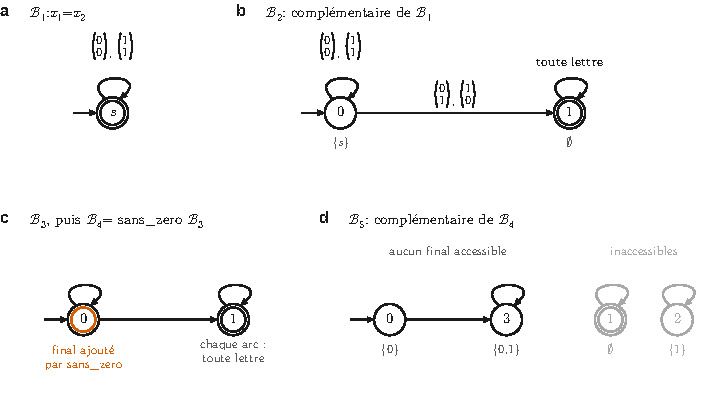
\includegraphics{figures/q27-deroule-automates.pdf}
\caption*{Figure 5 --- Déroulé sur φ(x₂) : ℬ₁, son complémentaire ℬ₂, la
projection ℬ₃ puis sans\_zero ℬ₄, et ℬ₅ sans état final accessible}
\end{figure}

\hypertarget{question-28}{%
\subsection{Question 28}\label{question-28}}

\begin{lstlisting}[language=Caml]
let rec automate_formule phi n =
  match phi with
  | Egale (V i, V j) -> automate_egalite n i j
  | Egale (V i, Plus (j, k)) -> automate_somme n j k i   (* v_j + v_k = v_i *)
  | Egale (Plus _, _) -> failwith "formule non sous forme simple"
  | Non psi -> complementaire (automate_formule psi n)
  | Et (psi1, psi2) ->
      intersection (automate_formule psi1 n) (automate_formule psi2 n)
  | Existe (i, psi) ->
      sans_zero (automate_existe (automate_formule psi n) i)
\end{lstlisting}

Chaque appel récursif porte sur une sous-formule stricte : le calcul termine. Toutes les fonctions employées conservent le champ \texttt{n}.

\hypertarget{question-29}{%
\subsection{Question 29}\label{question-29}}

On montre par induction structurelle la propriété suivante : pour toute formule \(\varphi\) sous forme simple de variables parmi \(x_1,\dots,x_n\), \(\mathcal{L}(\texttt{automate\_formule}\ \varphi\ n)=L_\varphi\). Rappelons que \(L_\varphi\) ne dépend que des lignes des variables libres ; les autres lignes sont quelconques.

\textbf{Lemme 1 (zéros à droite).} Pour tout \(m\) et tout \(j\), on a \(v_k(m{\mathbf{0}}^j)=v_k(m)\) pour tout \(k\) (on ajoute des bits de poids fort nuls). Donc \(a_{m{\mathbf{0}}^j}=a_m\).

\textbf{Lemme 2 (place pour un témoin).} Soit \(m\in\Sigma_n^*\), \(i\in[\![1,n]\!]\) et \(N\in\mathbb{N}\).

Il existe \(j\) et \(w\) avec \(|w|=|m|+j\), \(v_i(w)=N\) et \(\pi_k(w)=\pi_k(m{\mathbf{0}}^j)\) pour \(k\ne i\).

On prend \(j\) tel que \(2^{|m|+j}>N\), et pour ligne \(i\) l'écriture binaire de \(N\) sur \(|m|+j\) bits (Q2).

\textbf{Induction.}

\begin{itemize}
\tightlist
\item
  \textbf{\(x_i=x_j\)} : \texttt{automate\_egalite\ n\ i\ j} reconnaît \(\{m\mid v_i(m)=v_j(m)\}\), et \([\![x_i=x_j]\!]_{a_m}\) est vrai si et seulement si \(v_i(m)=v_j(m)\).
\item
  \textbf{\(x_i=x_j+x_k\)} : \texttt{automate\_somme\ n\ j\ k\ i} reconnaît \(\{m\mid v_j(m)+v_k(m)=v_i(m)\}=L_\varphi\).
\item
  \textbf{\(\neg\psi\)} : par Q12 et l'hypothèse d'induction, le langage est \(\Sigma_n^*\setminus L_\psi\). Comme \(\neg\psi\) et \(\psi\) ont les mêmes variables libres, \([\![\neg\psi]\!]_{a_m}\) est vrai si et seulement si \(m\notin L_\psi\).
\item
  \textbf{\(\psi_1\wedge\psi_2\)} : par Q13 et l'hypothèse d'induction, le langage est \(L_{\psi_1}\cap L_{\psi_2}\). Un même mot \(m\) fournit les valeurs des variables communes, et \(a_m\) restreinte aux variables libres de \(\psi_r\) est l'assignation de \(L_{\psi_r}\).
\item
  \textbf{\(\exists x_i.\psi\)} : soit \(\mathcal{C}=\texttt{automate\_existe}\ {\mathcal{A}}_\psi\ i\). Par Q25 et l'hypothèse d'induction, \(\mathcal{L}(\mathcal{C})=(L_\psi)_{\exists i}\). Par définition de \texttt{sans\_zero}, \(m\) est accepté si et seulement s'il existe \(j\ge0\) avec \(m{\mathbf{0}}^j\in(L_\psi)_{\exists i}\).

  \begin{itemize}
  \item
    (\(\subseteq\)) Soit \(w\in L_\psi\) qui coïncide avec \(m{\mathbf{0}}^j\) hors de la ligne \(i\).

    Le lemme 1 donne \(v_k(w)=v_k(m)\) pour \(k\ne i\).

    Donc \(\psi\) est vraie sous l'assignation qui donne \(v_k(m)\) aux autres variables libres et \(N:=v_i(w)\) à \(x_i\) : \([\![\exists x_i.\psi]\!]_{a_m}\) est vrai, et \(m\in L_\varphi\).
  \item
    (\(\supseteq\)) Si \(m\in L_\varphi\), il existe \(N\) tel que \(\psi\) soit vraie sous \(a_m\) modifiée par \(x_i\mapsto N\).

    Le lemme 2 fournit \(j\) et \(w\), et \(a_w\) est exactement cette assignation (lemme 1).

    Donc \(w\in L_\psi\), puis \(m{\mathbf{0}}^j\in(L_\psi)_{\exists i}\), et \(m\) est accepté.
  \end{itemize}
\end{itemize}

La forme simple ne contient ni \(\vee\), ni \(\to\), ni \(\forall\), et ses atomes ont l'une des deux formes traitées : \textbf{l'algorithme est correct}.

\hypertarget{question-30}{%
\subsection{Question 30}\label{question-30}}

\begin{lstlisting}[language=Caml]
let est_vraie phi n =
  let a = automate_formule phi n in
  a.finaux.(0)          (* l'état initial est l'état 0 *)
\end{lstlisting}

\textbf{Correction.} Si \(\varphi\) est close, l'assignation \(a_m\) est vide pour tout \(m\) : \(L_\varphi=\Sigma_n^*\) si \(\varphi\) est vraie, \(L_\varphi=\emptyset\) sinon.

Par Q29, l'automate reconnaît \(L_\varphi\).

Il n'y a pas de transition spontanée : \(\varepsilon\) est accepté si et seulement si l'état initial \(0\) est final. Donc \texttt{a.finaux.(0)} vaut \texttt{true} si et seulement si \(\varepsilon\in L_\varphi\), si et seulement si \textbf{\(\varphi\) est vraie}.

Le coût est celui de la construction de l'automate (exponentiel à chaque négation) ; la lecture finale est en \(O(1)\). Tautologie-Presburger est donc décidable.

\end{document}
